%
% Template LaTeX for 3 pages report of TI2P2
%
\documentclass[reprint, a4paper, nofootinbib, amsmath, amssymb, aps]{revtex4-1}
% 
%
\usepackage[english]{babel}
\usepackage[utf8]{inputenc}
%\usepackage{graphicx}
\usepackage{bm}
\usepackage[breaklinks]{hyperref}
\usepackage{amsmath}
\usepackage{mathrsfs}
\usepackage{amssymb}
\usepackage{float}
\usepackage{comment}
\usepackage{hyperref}
%\usepackage{mathtools}
% \newcommand*{\bfrac}[2]{\genfrac{}{}{0pt}{}{#1}{#2}}
%\usepackage{epstopdf}
\usepackage[pdftex]{graphicx,color}
%\epstopdfDeclareGraphicsRule{.pdf}{png}{.png}{convert #1 \OutputFile}
%\AppendGraphicsExtensions{.pdf}
% \usepackage{pdfpages} 
% \usepackage{lipsum}

\usepackage{caption}
\usepackage{tikz}
\usetikzlibrary{calc}
\usepackage{feynmf}
\usepackage{xcolor}
%\usepackage{etex}
\usepackage{textcomp}
\usepackage{marvosym}
\usepackage{wasysym}
\usepackage{amsthm}
\usepackage{comment}
\usepackage{qtree}
\usepackage{tikz-feynman}
\usepackage{array}
\usepackage[yyyymmdd]{datetime}
\begin{document}

\title{CHeat Sheet for new Ph.d student in the CMS team of IPHC}

\author{a Former Ph.d student}
\affiliation{Université de Strasbourg, IPHC, 23 rue du Loess 67037 Strasbourg, France}

\date{\today}

\maketitle

%%%%%%%%%%%%%%%%%%%
\section{Introduction}

First and foremost, welcome to the CMS team of Strasbourg and congratulation for being promoted to Ph.D student (or intern). This paper will try to quickly give you tools and useful links to better understand what are all the acronyms that you may encounter, LaTeX related things, CMS related things, etc (Nothing related to the Ecole Doctoral will be mentioned as rules given may change over years...). This list won't be exhaustive as there so many things to talk about but we hope that this will help you n any kind of way to fasten your progress in your work. Good luck!  

\section{Acronyms}
    A set of Acronyms is defined in a Twiki page in : \href{https://twiki.cern.ch/twiki/bin/view/CMSPublic/WorkBookGlossary}{TwikiAcronyms}. Twiki pages are like wiki pages but for the CMS documentation of everything. By the time you read this, this may have changed to gitlab or something else.
%%%%%%%%%%%%%%%%%%%
\section{Compact Muon Solenoid detector }
    
    %----------------%
    \subsection{Point 5}

    The CMS detector is situated at one of the crossing point between the two beams of the LHC, also called Point 5 or P5. During your Ph.D, you will have to perform shift at P5 (trigger shifts, Data Quality Monitoring (DQM), Shift Leader, Data Acquisition System (DAQ), DCS Detector Control Status). There are different types of shifts, online (usually at P5) and offline (can be performed outside of P5 usually). A shift last 8 hours where you take care of one aspect of the detector mentioned above and have to communicate important information to others, the shift leader especially.
    It may change over time but a certain amount of shifts have to be performed by the CMS team of IPHC (there are quotas) and usually online shifts are the ones that are done to fulfill the quotas (even more points when doing night shifts). All the links related to the different shifts will not be given here as they may be updated quite often and are really specific. No worries, everything will be given to you by shifts coordinators when the time will come. \\
    Personal Experience: Trigger Shifts and DQM shifts are pretty cool and all kinds of shift help you better understand the experiment
    
    PS: Becareful, P5 is NOT on the Meyrin or the Prevessin sites. You need to take your car or the shuttle to get to P5 as CMS is wondering around in the countryside. There is also the car-sharing system of CMS. Taking the bike is not really recommended.
    


    \subsection{The detector}
    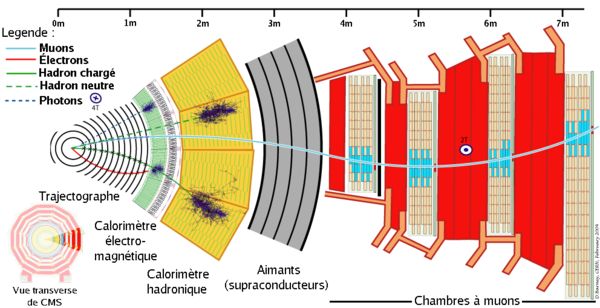
\includegraphics[height=4cm, width=8cm, trim= 0cm 0cm 0cm 0cm,clip]{Images/cmsAll.png}
    \label{fig: CMS}
    The CMS detector is 15 meter wide and 21 meter long. You can see a transverse view of CMS in Fig.\ref{fig: CMS}. The description will be a bit biased since the Strasbourg team is highly involved in the current tracker and its upgrade. At the very center, the closes part with respect to the interaction point is the beam pipe.Then comes the tracker that is divided into two parts (see Fig.\ref{fig: Tracker}) : Pixels and strips. Pixels are the innermost part of the tracker and also divided in to two parts: Barrel Pixels (BPIX) and Forward Pixels (FPIX). After the Pixels are the strips also divided into several parts: Tracker Inner Barrel (TIB), Tracker Outer Barrel (TOB). Then, there the two forward parts : the Tracker Inner Disks (TID) and Tracker End Caps (TEC). The characteristics (pitch, width, etc) of the modules of the silicon strip tracker change depending on where there are in the tracker.
    For the tracking, an iterative process is implemented to look for tracks. For electrons, it's slightly different due to Bremsstrahlung, the tracking is using the GaussianSum filter to take into account the information of photons. You may therefore encounter GSF electrons when coding :D. THe goal of the tracker is to reconstruct the tracks of charged particles (that deposits energy in the layers of the tracker)\\
    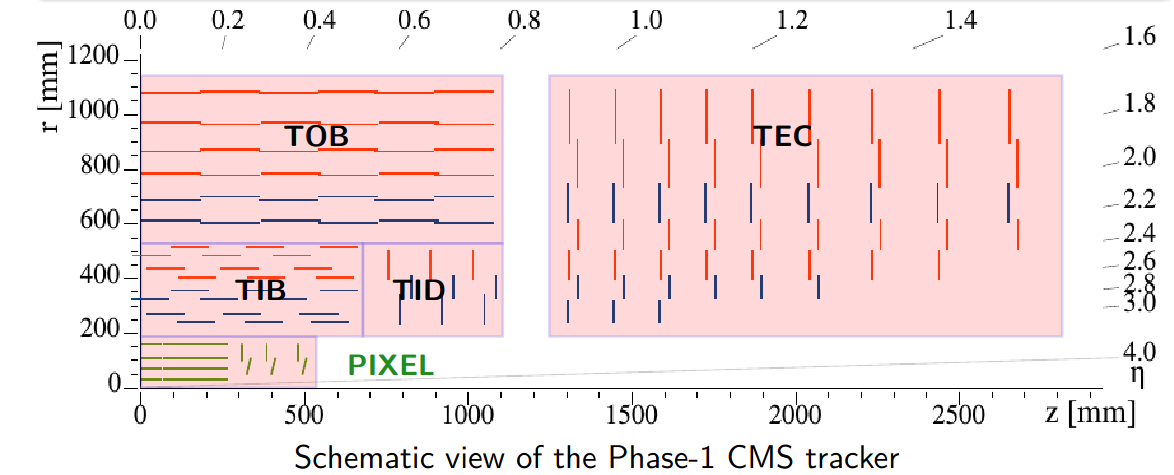
\includegraphics[height=4cm, width=8cm, trim= 0cm 0cm 0cm 0cm,clip]{Images/CMSTracker.png}\label{fig: Tracker}
    After the tracker comes the Electromagnetic and hadronic calorimeters. The former is used to detect energy deposits from photons and electrons (used for the GSF tracking). The hadronic calorimeter is used to detect energy deposits from both neutral and charged hadrons. \\
    Finally, there are the muons chambers. Again there are different types of subdetector for muon chambers like Resistive Plate Chambers (RPCs), Cathode Strip Chambers (CSC), Gas Electron Multiplier (GEM), Drift Tubes (DTs).Here is a small document to explain how each one of them works : \href{https://cds.cern.ch/record/2698492/files/Poster-2019-989.pdf}{Muon Poster} (click on Muon Poster).

    Since you are working in the Strasbourg team, some part of your work may be related to the tracker, here are a few links to better understand the tracker :
    \begin{itemize}
        \item \href{https://indico.cern.ch/event/1238081/timetable/#20230227}{Tracker training days 2023} : a lot of slides about everything concerning pixels and strips
        \item If you like reading more than going through slides, here is \href{https://cds.cern.ch/record/914891/files/jpconf6_41_011.pdf}{Doc Tracker}. Quite old but gives the basics
        \item Quantities related to the tracker : \href{http://cms.cern.ch/iCMS/jsp/openfile.jsp?type=DN&year=2020&files=DN2020_004.pdf}{Click}
    \end{itemize}
    
%%%%%%%%%%%%%%%%%%%
\section{LaTeX}
    You might need to use some LaTeX during your Ph.D, only examples will be given and a cheat sheet :
    \begin{itemize}
        \item \href{https://wch.github.io/latexsheet/}{Cheat Sheet}
        \item FeynMan Diagrams : examples are given in the twiki page, see ppToXX 
        \item Poster : an exemple is given 
        \item  \textcolor{red}{to be added}
    \end{itemize}

    You will see that the TikZ library is used and is kinda common to draw shapes, add things to already existing plots, Feynman diagrams, etc. When using the tikzFeynman library or tikz in general, you may need to change the compiler of overleaf to lualatex in the Menu on the top left.
\section{root}

 Only few things will be given as there are not much things to know  about ROOT.
 Be always careful about the version of root you are using as you may face root version incompatibility. You can change the version of root you are using by doing this command  on the uiX: \\
 \begin{center}
     $\rightarrow$ ls  /libcern/root (to check which version are available) \\
     $\rightarrow$ source /libcern/root/6.24.06/centos7.6-x86\_64/bin/thisroot.sh to change of version (for example)
 \end{center}
 
\section{Physics Analysis}
Madgraph / generation, pythia8, powheg

Gen-Sim, Raw, reco, AOD, MniAOD, Nanoaod
\subsection{Run 2}
\subsection{Run 3}
\subsection{Physics Object}
\subsubsection{Muons}
    \subsubsection{Electrons}
    \subsubsection{Photons}
\subsection{Tracks}

\subsection{Analysis Strategy}

\subsection{Combine}

\subsection{Publication}
%%%%%%%%%%%%%%%%%%%

%%%%%%%%%%%%%%%%%%%%%%%%%%%%%%

\end{document}
